\chapter{Ergebnisse}
\label{chap:ergebnisse} Dieses Kapitel präsentiert alle Ergebnisse, die in
dieser Arbeit erzielt wurde. Dabei spielen nicht nur die erfolgreichen Ziele eine
Rolle, sondern auch die Misserfolge. Zunächst wird die entwickelte Erweiterung in
seiner finalen Form beschrieben, gefolgt von einer Darstellung der zentralen
Funktionen. Anschließend wird auf die Konzeptionen und Umsetzungen der verschiedenen
Teile eingegangen. Abschließend soll die Performance und die verschiedenen
Anwendungsszenarien genauer analysiert werden. Daraus ergeben sich auch Limitierungen
für die Software. Mit diesen erstellten Analysen kann unter Berücksichtigung
eine Aussage bezogen auf die Forschungsfrage gestellt werden.
% ---------------------------------------------------------------------------------------

\section{Tooth Analyser}
Im Rahmen dieser vorliegenden Arbeit ist eine 3D Slicer Extension entstanden, die
den Namen Tooth Analyser trägt und für die Forschung im Dentalbereich eingesetzt
wird. In erster Linie können mit diesem Plugin Micro CT Aufnahmen anatomisch
segmentiert werden. Das Modul schmiegt sich wie alle anderen Module gut in die Kernanwendung
ein und bietet eine \ac{UI}. Neben der eigentlichen Implementierung ist auch ein
Logo für das Plugin entstanden, das es nach außen repräsentiert. Die Abbildung \ref{fig:logo_tooth_analyser}
zeigt dies.

\begin{figure}[h]
	\centering
	
\includegraphics[width=0.9\textwidth]{img/SlicerToothAnalyser.png}
	\caption{Logo der 3D Slicer Erweiterung "Tooth Analyser", welche im Rahmen dieser
	Arbeit entwickelt wurde. Logodesign: Dr. Elias Walter}
	\label{fig:logo_tooth_analyser}
\end{figure}

Des Emblem des Tooth Analyser bildet einen Zahn ab, dessen Hauptsegmenten (Schmelz,
Dentin, Pulpa) mit den unterschiedlichen Farben (grün, gelb, orange) visualisiert
werden. Dies verdeutlicht die Analogie zur anatomischen Segmentierung und lässt
gleich vermuten, dass sich dieses Modul mit einer Segmentierung beschäftigt. Der
Untertitel des Logos lässt darauf deuten, dass es um die Segmentierung von Micro
\ac{CT} Aufnahmen geht. Wurde der Tooth Analyser installiert, so ist er über den
Menüpunkt Module in Slicer auswählbar. Hier wird er in dem Unterpunkt \textit{Segmentierung}
eingruppiert, was ein weiteres Indiz auf die grobe Funktionalität liefert. Wird
also der Tooth Analyser gestartet so erhält man die Ansicht der Kernanwendung
mit der Entsprechenden \ac{UI}. Die Abbildung \ref{fig:tooth_analyser_start_up}
soll genau diese Ansicht verdeutlichen

\begin{figure}[h]
	\centering
	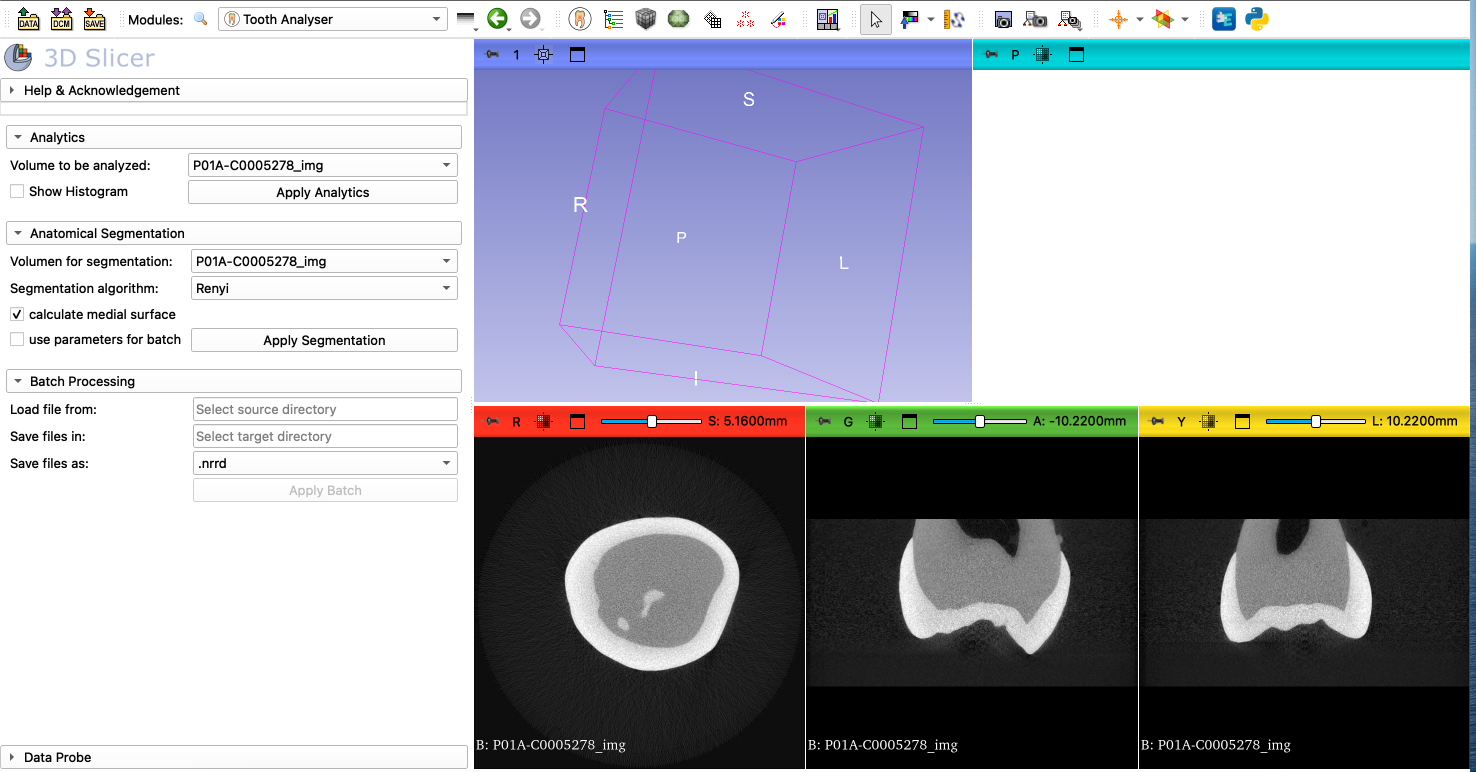
\includegraphics[scale=0.2, width=\textwidth]{img/toothAnalyserStarUp.png}
	\caption{Startansicht der Erweiterung Tooth Analyser nach dem ersten Aufruf}
	\label{fig:tooth_analyser_start_up}
\end{figure}

Die Ansicht zeigt die Kernanwendung (rechts die verschiedenen Fenster) und die
\ac{UI} des jeweiligen Moduls. Die Kernanwendung kann auch als Szene beschrieben
werden und übernimmt alle generischen Handhabungen der Bilder. Neben den Szenen ist
auch immer eine Sidebar zu sehen, welche die \ac{UI} des jeweiligen Moduls abbildet.
Im Falle der Abbildung \ref{fig:tooth_analyser_start_up} ist es die \ac{UI} des Tooth
Analyser. Das manuelle Laden eines Bildes in die Szene ist Teil der Slicer
Kernanwendung und nicht teil der Modullogik. Das bereits geladene Bild ist demnach
unabhängig von der Slicer Erweiterung entstanden. Betrachtet man die
Benutzerschnittstelle genauer, so fällt sofort auf, dass diese in vier Bereiche
unterteilt ist. Der Bereich \textit{Help and Acknowledgement} stellt Hilfen und
Informationen über das Modul bereit. Über diesen Abschnitt ist auch die offizielle
Dokumentation über dieses Modul erreichbar. Zu Beachten ist, dass dieser Bereich
nicht eigens für den Tooth Analyser entwickelt wurde. Es handelt sich hier um
eine Funktionalität, die automatisch allen \ac{SEM} zur Verfügung steht. Bei den
übrigen Abschnitten handelt es sich im Features die spezifische für den Tooth Analyser
entwickelt wurden. Bevor genauer auf die Funktionalitäten des Tooth Analyser
eingegangen wird, sei zunächst auf die Abbildung ... verwiesen, welche die
Kernfunktionalitäten zeigt.

\begin{figure}[h]
	\centering
	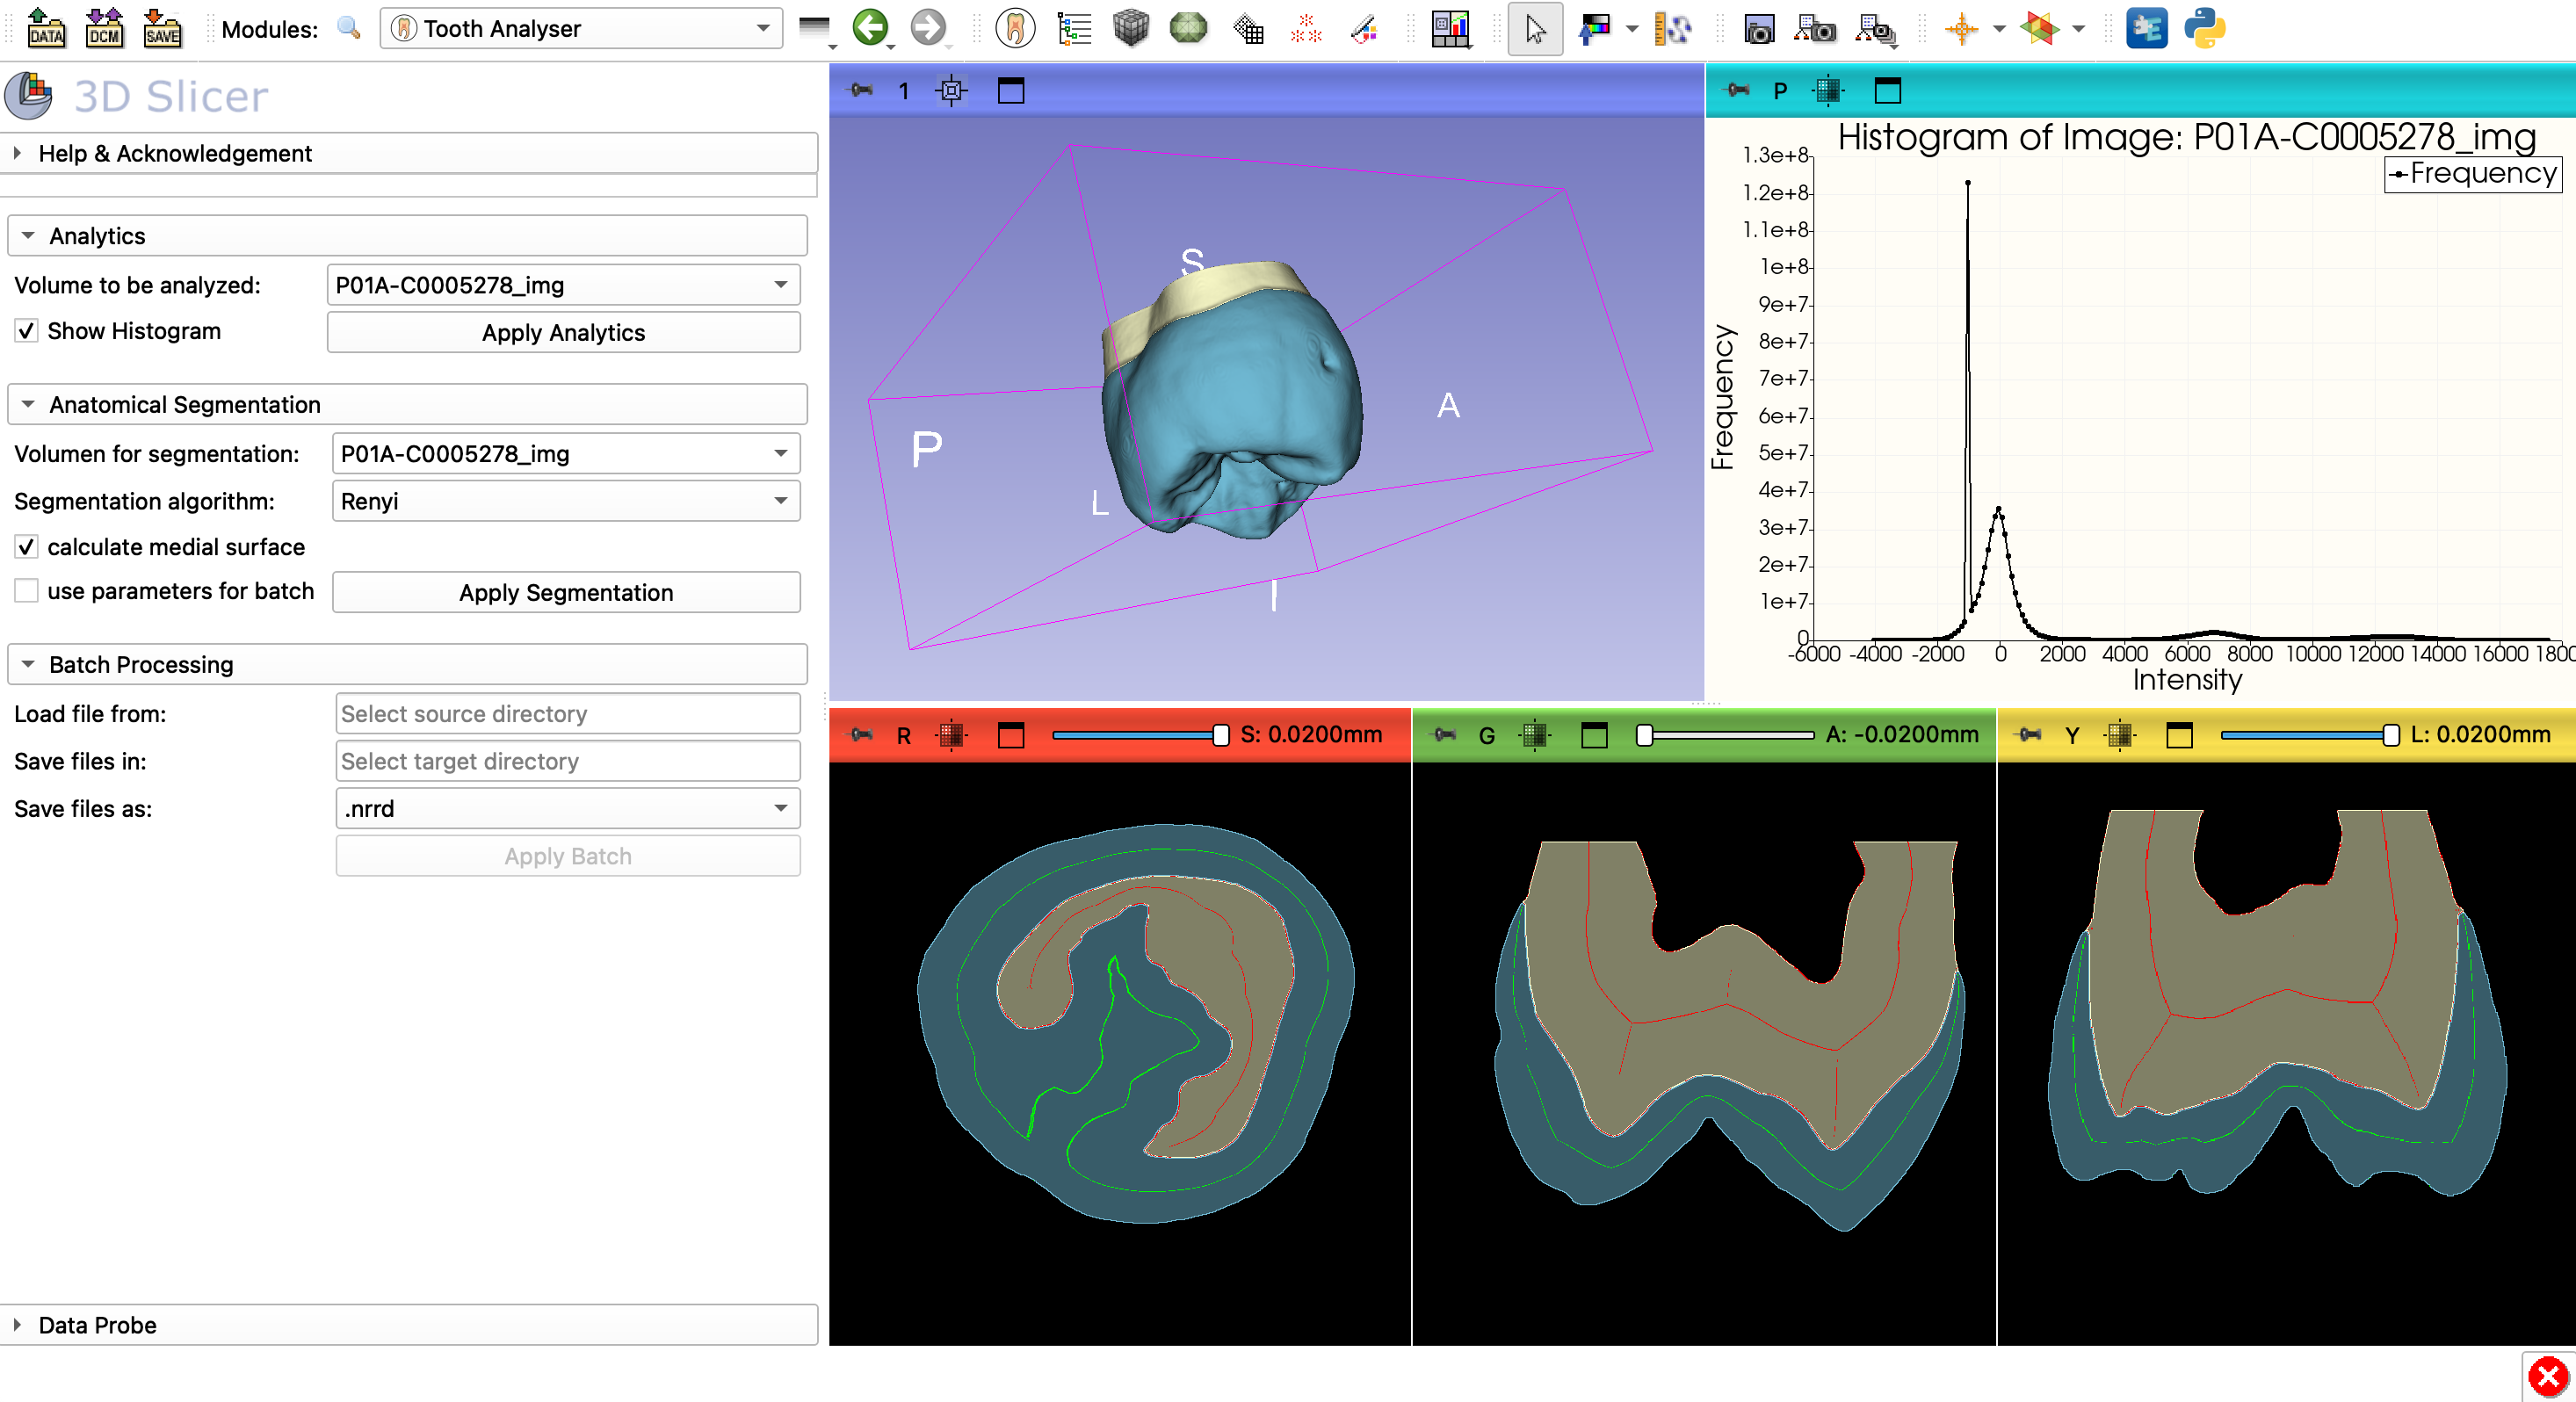
\includegraphics[scale=0.2, width=\textwidth]{img/toothAnalyserFullView.png}
	\caption{Ergebnisansicht der Erweiterung Tooth Analyser nachdem die Analysen
	und die anatomische Segmentierung erstellt wurden.}
	\label{fig:tooth_analyser_full_view}
\end{figure}

Der Analysebereich des Tooth Analyser ermöglicht es das Histogramm eines gegebenen
Bildes zu erstellen. Dies ist besonders interessant, wenn ein segmentierungs Algortihmus
ausgewählt werden muss. Diese Algorithmen sind Schwellwertverfahren, die auf das
Histogramm eines Bildes basieren, um es zu segmentieren. Das erstellte Histogramm
ist rechts oben in der Abbildung \ref{fig:tooth_analyser_full_view} zu erkennen.
Es wird in einem Plot-Node dargestellt und kann über diesn auch verändert werden.
Hierzu ist die Pinnadel im fenster des Plot-Node zu wählen. Durch die
Speicherfunktion der Kernanwendung kann diese Funktion auch problemlos
gespeichert werden. Über das Modul \textit{Data} kann auch der Name des
Diagramms verändert werden.

- hier noch die Parameter beschreiben

- erzählen, dass nur scalarnode ausgewählt werden

- es wird das erste node genommen, dass geladen wird um klicks zu sparen

- apply ist ausgegraut, biss alle parameter eingestellt sind und sinn ergeben

Die Hauptfunktionalität des Tooth Analyser ist die anatomische Segmentierung welche
in Kapitel \ref{sec:verwwandte_arbeit} detaliert erläutert wurde. Diese sieht
drei Parameter vor, die eingestellt werden müssen. Um die Komplexität gering zu
halten und schnell zu einem Ergebnis zu kommen, wurde bewusst auf viele Parameter
verzichtet und eine Vorauswahl implementiert.

- hier die Parameter beschreiben

- erzählen, dass nur scalarnode ausgewählt werden

- es wird das erste node genommen, dass geladen wird um klicks zu sparen

- apply ist ausgegraut, biss alle parameter eingestellt sind und sinn ergeben

- was beinhaltet das Modul noch (Analytics)

- Screenshot der UI

% ---------------------------------------------------------------------------------------

\section{Konzeptionen}
- Wireframes

- Klassendiagramme
% ---------------------------------------------------------------------------------------

\section{Technische Umsetzung}
- ichtige Codeausschnitte

- Das logic interface

- die aufteilung in Module
% ---------------------------------------------------------------------------------------

\section{Performance}
Die Laufzeitanalyse des Systems.
% ---------------------------------------------------------------------------------------

\section{Anwendungsszenarien}
Wie wird das tool eingesetzt, wer setzt es ein, Segmentierung des gazen Zahnes
ist auch möglich.

- Segmentieren

- überlappen der asnzeige mit Medialflächen

% ---------------------------------------------------------------------------------------

\section{Limitierungen}

- kleine bilder

- preprocessing
% ---------------------------------------------------------------------------------------